\documentclass[1p]{elsarticle_modified}
%\bibliographystyle{elsarticle-num}

%\usepackage[colorlinks]{hyperref}
%\usepackage{abbrmath_seonhwa} %\Abb, \Ascr, \Acal ,\Abf, \Afrak
\usepackage{amsfonts}
\usepackage{amssymb}
\usepackage{amsmath}
\usepackage{amsthm}
\usepackage{scalefnt}
\usepackage{amsbsy}
\usepackage{kotex}
\usepackage{caption}
\usepackage{subfig}
\usepackage{color}
\usepackage{graphicx}
\usepackage{xcolor} %% white, black, red, green, blue, cyan, magenta, yellow
\usepackage{float}
\usepackage{setspace}
\usepackage{hyperref}

\usepackage{tikz}
\usetikzlibrary{arrows}

\usepackage{multirow}
\usepackage{array} % fixed length table
\usepackage{hhline}

%%%%%%%%%%%%%%%%%%%%%
\makeatletter
\renewcommand*\env@matrix[1][\arraystretch]{%
	\edef\arraystretch{#1}%
	\hskip -\arraycolsep
	\let\@ifnextchar\new@ifnextchar
	\array{*\c@MaxMatrixCols c}}
\makeatother %https://tex.stackexchange.com/questions/14071/how-can-i-increase-the-line-spacing-in-a-matrix
%%%%%%%%%%%%%%%

\usepackage[normalem]{ulem}

\newcommand{\msout}[1]{\ifmmode\text{\sout{\ensuremath{#1}}}\else\sout{#1}\fi}
%SOURCE: \msout is \stkout macro in https://tex.stackexchange.com/questions/20609/strikeout-in-math-mode

\newcommand{\cancel}[1]{
	\ifmmode
	{\color{red}\msout{#1}}
	\else
	{\color{red}\sout{#1}}
	\fi
}

\newcommand{\add}[1]{
	{\color{blue}\uwave{#1}}
}

\newcommand{\replace}[2]{
	\ifmmode
	{\color{red}\msout{#1}}{\color{blue}\uwave{#2}}
	\else
	{\color{red}\sout{#1}}{\color{blue}\uwave{#2}}
	\fi
}

\newcommand{\Sol}{\mathcal{S}} %segment
\newcommand{\D}{D} %diagram
\newcommand{\A}{\mathcal{A}} %arc


%%%%%%%%%%%%%%%%%%%%%%%%%%%%%5 test

\def\sl{\operatorname{\textup{SL}}(2,\Cbb)}
\def\psl{\operatorname{\textup{PSL}}(2,\Cbb)}
\def\quan{\mkern 1mu \triangleright \mkern 1mu}

\theoremstyle{definition}
\newtheorem{thm}{Theorem}[section]
\newtheorem{prop}[thm]{Proposition}
\newtheorem{lem}[thm]{Lemma}
\newtheorem{ques}[thm]{Question}
\newtheorem{cor}[thm]{Corollary}
\newtheorem{defn}[thm]{Definition}
\newtheorem{exam}[thm]{Example}
\newtheorem{rmk}[thm]{Remark}
\newtheorem{alg}[thm]{Algorithm}

\newcommand{\I}{\sqrt{-1}}
\begin{document}

%\begin{frontmatter}
%
%\title{Boundary parabolic representations of knots up to 8 crossings}
%
%%% Group authors per affiliation:
%\author{Yunhi Cho} 
%\address{Department of Mathematics, University of Seoul, Seoul, Korea}
%\ead{yhcho@uos.ac.kr}
%
%
%\author{Seonhwa Kim} %\fnref{s_kim}}
%\address{Center for Geometry and Physics, Institute for Basic Science, Pohang, 37673, Korea}
%\ead{ryeona17@ibs.re.kr}
%
%\author{Hyuk Kim}
%\address{Department of Mathematical Sciences, Seoul National University, Seoul 08826, Korea}
%\ead{hyukkim@snu.ac.kr}
%
%\author{Seokbeom Yoon}
%\address{Department of Mathematical Sciences, Seoul National University, Seoul, 08826,  Korea}
%\ead{sbyoon15@snu.ac.kr}
%
%\begin{abstract}
%We find all boundary parabolic representation of knots up to 8 crossings.
%
%\end{abstract}
%\begin{keyword}
%    \MSC[2010] 57M25 
%\end{keyword}
%
%\end{frontmatter}

%\linenumbers
%\tableofcontents
%
\newcommand\colored[1]{\textcolor{white}{\rule[-0.35ex]{0.8em}{1.4ex}}\kern-0.8em\color{red} #1}%
%\newcommand\colored[1]{\textcolor{white}{ #1}\kern-2.17ex	\textcolor{white}{ #1}\kern-1.81ex	\textcolor{white}{ #1}\kern-2.15ex\color{red}#1	}

{\Large $\underline{12a_{1234}~(K12a_{1234})}$}

\setlength{\tabcolsep}{10pt}
\renewcommand{\arraystretch}{1.6}
\vspace{1cm}\begin{tabular}{m{100pt}>{\centering\arraybackslash}m{274pt}}
\multirow{5}{120pt}{
	\centering
	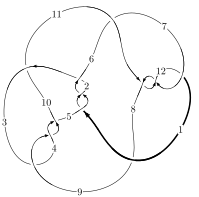
\includegraphics[width=112pt]{../../../GIT/diagram.site/Diagrams/png/2035_12a_1234.png}\\
\ \ \ A knot diagram\footnotemark}&
\allowdisplaybreaks
\textbf{Linearized knot diagam} \\
\cline{2-2}
 &
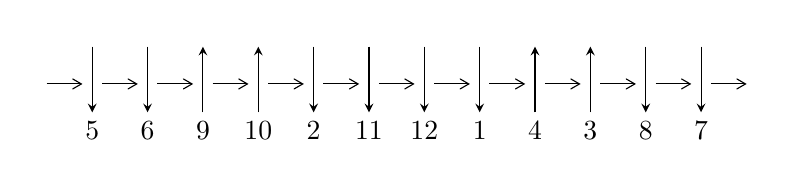
\begin{tikzpicture}[x=20pt, y=17pt]
	% nodes
	\node (C0) at (0, 0) {};
	\node (C1) at (1, 0) {};
	\node (C1U) at (1, +1) {};
	\node (C1D) at (1, -1) {5};

	\node (C2) at (2, 0) {};
	\node (C2U) at (2, +1) {};
	\node (C2D) at (2, -1) {6};

	\node (C3) at (3, 0) {};
	\node (C3U) at (3, +1) {};
	\node (C3D) at (3, -1) {9};

	\node (C4) at (4, 0) {};
	\node (C4U) at (4, +1) {};
	\node (C4D) at (4, -1) {10};

	\node (C5) at (5, 0) {};
	\node (C5U) at (5, +1) {};
	\node (C5D) at (5, -1) {2};

	\node (C6) at (6, 0) {};
	\node (C6U) at (6, +1) {};
	\node (C6D) at (6, -1) {11};

	\node (C7) at (7, 0) {};
	\node (C7U) at (7, +1) {};
	\node (C7D) at (7, -1) {12};

	\node (C8) at (8, 0) {};
	\node (C8U) at (8, +1) {};
	\node (C8D) at (8, -1) {1};

	\node (C9) at (9, 0) {};
	\node (C9U) at (9, +1) {};
	\node (C9D) at (9, -1) {4};

	\node (C10) at (10, 0) {};
	\node (C10U) at (10, +1) {};
	\node (C10D) at (10, -1) {3};

	\node (C11) at (11, 0) {};
	\node (C11U) at (11, +1) {};
	\node (C11D) at (11, -1) {8};

	\node (C12) at (12, 0) {};
	\node (C12U) at (12, +1) {};
	\node (C12D) at (12, -1) {7};
	\node (C13) at (13, 0) {};

	% arrows
	\draw[->,>={angle 60}]
	(C0) edge (C1) (C1) edge (C2) (C2) edge (C3) (C3) edge (C4) (C4) edge (C5) (C5) edge (C6) (C6) edge (C7) (C7) edge (C8) (C8) edge (C9) (C9) edge (C10) (C10) edge (C11) (C11) edge (C12) (C12) edge (C13) ;	\draw[->,>=stealth]
	(C1U) edge (C1D) (C2U) edge (C2D) (C3D) edge (C3U) (C4D) edge (C4U) (C5U) edge (C5D) (C6U) edge (C6D) (C7U) edge (C7D) (C8U) edge (C8D) (C9D) edge (C9U) (C10D) edge (C10U) (C11U) edge (C11D) (C12U) edge (C12D) ;
	\end{tikzpicture} \\
\hhline{~~} \\& 
\textbf{Solving Sequence} \\ \cline{2-2} 
 &
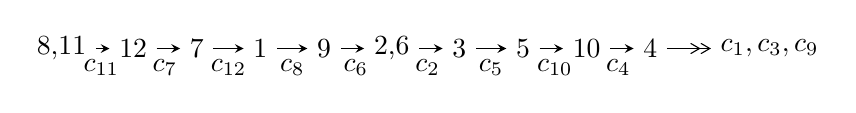
\begin{tikzpicture}[x=23pt, y=7pt]
	% node
	\node (A0) at (-1/8, 0) {8,11};
	\node (A1) at (1, 0) {12};
	\node (A2) at (2, 0) {7};
	\node (A3) at (3, 0) {1};
	\node (A4) at (4, 0) {9};
	\node (A5) at (81/16, 0) {2,6};
	\node (A6) at (49/8, 0) {3};
	\node (A7) at (57/8, 0) {5};
	\node (A8) at (65/8, 0) {10};
	\node (A9) at (73/8, 0) {4};
	\node (C1) at (1/2, -1) {$c_{11}$};
	\node (C2) at (3/2, -1) {$c_{7}$};
	\node (C3) at (5/2, -1) {$c_{12}$};
	\node (C4) at (7/2, -1) {$c_{8}$};
	\node (C5) at (9/2, -1) {$c_{6}$};
	\node (C6) at (45/8, -1) {$c_{2}$};
	\node (C7) at (53/8, -1) {$c_{5}$};
	\node (C8) at (61/8, -1) {$c_{10}$};
	\node (C9) at (69/8, -1) {$c_{4}$};
	\node (A10) at (11, 0) {$c_{1},c_{3},c_{9}$};

	% edge
	\draw[->,>=stealth]	
	(A0) edge (A1) (A1) edge (A2) (A2) edge (A3) (A3) edge (A4) (A4) edge (A5) (A5) edge (A6) (A6) edge (A7) (A7) edge (A8) (A8) edge (A9) ;
	\draw[->>,>={angle 60}]	
	(A9) edge (A10);
\end{tikzpicture} \\ 

\end{tabular} \\

\footnotetext{
The image of knot diagram is generated by the software ``\textbf{Draw programme}" developed by Andrew Bartholomew(\url{http://www.layer8.co.uk/maths/draw/index.htm\#Running-draw}), where we modified some parts for our purpose(\url{https://github.com/CATsTAILs/LinksPainter}).
}\phantom \\ \newline 
\centering \textbf{Ideals for irreducible components\footnotemark of $X_{\text{par}}$} 
 
\begin{align*}
I^u_{1}&=\langle 
1.93075\times10^{22} u^{71}-9.36918\times10^{22} u^{70}+\cdots+2.61600\times10^{23} b-2.51001\times10^{23},\\
\phantom{I^u_{1}}&\phantom{= \langle  }3.91390\times10^{23} u^{71}-8.79983\times10^{23} u^{70}+\cdots+2.61600\times10^{23} a-2.96665\times10^{24},\;u^{72}-2 u^{71}+\cdots-8 u-1\rangle \\
I^u_{2}&=\langle 
- a u- u^2+b+u-1,\;a^2-4 u^2+2 u-6,\;u^3- u^2+2 u-1\rangle \\
I^u_{3}&=\langle 
- u^2+b- u-1,\;a,\;u^3+u^2+2 u+1\rangle \\
\\
\end{align*}
\raggedright * 3 irreducible components of $\dim_{\mathbb{C}}=0$, with total 81 representations.\\
\footnotetext{All coefficients of polynomials are rational numbers. But the coefficients are sometimes approximated in decimal forms when there is not enough margin.}
\newpage
\renewcommand{\arraystretch}{1}
\centering \section*{I. $I^u_{1}= \langle 1.93\times10^{22} u^{71}-9.37\times10^{22} u^{70}+\cdots+2.62\times10^{23} b-2.51\times10^{23},\;3.91\times10^{23} u^{71}-8.80\times10^{23} u^{70}+\cdots+2.62\times10^{23} a-2.97\times10^{24},\;u^{72}-2 u^{71}+\cdots-8 u-1 \rangle$}
\flushleft \textbf{(i) Arc colorings}\\
\begin{tabular}{m{7pt} m{180pt} m{7pt} m{180pt} }
\flushright $a_{8}=$&$\begin{pmatrix}0\\u\end{pmatrix}$ \\
\flushright $a_{11}=$&$\begin{pmatrix}1\\0\end{pmatrix}$ \\
\flushright $a_{12}=$&$\begin{pmatrix}1\\u^2\end{pmatrix}$ \\
\flushright $a_{7}=$&$\begin{pmatrix}u\\u^3+u\end{pmatrix}$ \\
\flushright $a_{1}=$&$\begin{pmatrix}u^2+1\\u^4+2 u^2\end{pmatrix}$ \\
\flushright $a_{9}=$&$\begin{pmatrix}- u^5-2 u^3- u\\- u^7-3 u^5-2 u^3+u\end{pmatrix}$ \\
\flushright $a_{2}=$&$\begin{pmatrix}-1.49614 u^{71}+3.36385 u^{70}+\cdots+9.35049 u+11.3404\\-0.0738055 u^{71}+0.358149 u^{70}+\cdots-1.96687 u+0.959482\end{pmatrix}$ \\
\flushright $a_{6}=$&$\begin{pmatrix}u^3+2 u\\u^3+u\end{pmatrix}$ \\
\flushright $a_{3}=$&$\begin{pmatrix}-1.70670 u^{71}+4.43356 u^{70}+\cdots+11.3889 u+11.8788\\-0.0934270 u^{71}+1.10929 u^{70}+\cdots-1.29641 u+1.19703\end{pmatrix}$ \\
\flushright $a_{5}=$&$\begin{pmatrix}0.959482 u^{71}-1.99277 u^{70}+\cdots-1.06519 u-9.64273\\0.371572 u^{71}-0.601476 u^{70}+\cdots-0.628716 u-1.49614\end{pmatrix}$ \\
\flushright $a_{10}=$&$\begin{pmatrix}-2.52657 u^{71}+5.46669 u^{70}+\cdots+6.75726 u+15.3627\\-0.515104 u^{71}+0.594756 u^{70}+\cdots+2.97411 u+2.22254\end{pmatrix}$ \\
\flushright $a_{4}=$&$\begin{pmatrix}-1.82146 u^{71}+4.39966 u^{70}+\cdots+11.3717 u+12.1549\\0.225358 u^{71}+0.517327 u^{70}+\cdots-1.91838 u+0.946928\end{pmatrix}$\\&\end{tabular}
\flushleft \textbf{(ii) Obstruction class $= -1$}\\~\\
\flushleft \textbf{(iii) Cusp Shapes $= \frac{131451318810141352881632}{130800077995111299411101} u^{71}-\frac{277192896356154580549909}{130800077995111299411101} u^{70}+\cdots+\frac{732571967736991836052242}{130800077995111299411101} u+\frac{336112699848274877396314}{130800077995111299411101}$}\\~\\
\newpage\renewcommand{\arraystretch}{1}
\flushleft \textbf{(iv) u-Polynomials at the component}\newline \\
\begin{tabular}{m{50pt}|m{274pt}}
Crossings & \hspace{64pt}u-Polynomials at each crossing \\
\hline $$\begin{aligned}c_{1},c_{2},c_{5}\end{aligned}$$&$\begin{aligned}
&u^{72}+4 u^{71}+\cdots+51 u-7
\end{aligned}$\\
\hline $$\begin{aligned}c_{3},c_{4},c_{9}\end{aligned}$$&$\begin{aligned}
&u^{72}- u^{71}+\cdots+8 u-8
\end{aligned}$\\
\hline $$\begin{aligned}c_{6},c_{8}\end{aligned}$$&$\begin{aligned}
&u^{72}-2 u^{71}+\cdots+5260 u-481
\end{aligned}$\\
\hline $$\begin{aligned}c_{7},c_{11},c_{12}\end{aligned}$$&$\begin{aligned}
&u^{72}+2 u^{71}+\cdots+8 u-1
\end{aligned}$\\
\hline $$\begin{aligned}c_{10}\end{aligned}$$&$\begin{aligned}
&u^{72}+3 u^{71}+\cdots-2888 u-5768
\end{aligned}$\\
\hline
\end{tabular}\\~\\
\newpage\renewcommand{\arraystretch}{1}
\flushleft \textbf{(v) Riley Polynomials at the component}\newline \\
\begin{tabular}{m{50pt}|m{274pt}}
Crossings & \hspace{64pt}Riley Polynomials at each crossing \\
\hline $$\begin{aligned}c_{1},c_{2},c_{5}\end{aligned}$$&$\begin{aligned}
&y^{72}-70 y^{71}+\cdots+423 y+49
\end{aligned}$\\
\hline $$\begin{aligned}c_{3},c_{4},c_{9}\end{aligned}$$&$\begin{aligned}
&y^{72}-65 y^{71}+\cdots-448 y+64
\end{aligned}$\\
\hline $$\begin{aligned}c_{6},c_{8}\end{aligned}$$&$\begin{aligned}
&y^{72}-52 y^{71}+\cdots-12759486 y+231361
\end{aligned}$\\
\hline $$\begin{aligned}c_{7},c_{11},c_{12}\end{aligned}$$&$\begin{aligned}
&y^{72}+60 y^{71}+\cdots-62 y+1
\end{aligned}$\\
\hline $$\begin{aligned}c_{10}\end{aligned}$$&$\begin{aligned}
&y^{72}+19 y^{71}+\cdots-312337216 y+33269824
\end{aligned}$\\
\hline
\end{tabular}\\~\\
\newpage\flushleft \textbf{(vi) Complex Volumes and Cusp Shapes}
$$\begin{array}{c|c|c}  
\text{Solutions to }I^u_{1}& \I (\text{vol} + \sqrt{-1}CS) & \text{Cusp shape}\\
 \hline 
\begin{aligned}
u &= -0.855221 + 0.104555 I \\
a &= -3.51455 - 0.94548 I \\
b &= -2.90722 - 0.53414 I\end{aligned}
 & -11.19460 + 5.99079 I & -11.45914 - 4.34329 I \\ \hline\begin{aligned}
u &= -0.855221 - 0.104555 I \\
a &= -3.51455 + 0.94548 I \\
b &= -2.90722 + 0.53414 I\end{aligned}
 & -11.19460 - 5.99079 I & -11.45914 + 4.34329 I \\ \hline\begin{aligned}
u &= \phantom{-}0.846928 + 0.141420 I \\
a &= -3.30013 + 1.21203 I \\
b &= -2.78162 + 0.68434 I\end{aligned}
 & -5.95434 - 10.47780 I & -7.43345 + 6.18173 I \\ \hline\begin{aligned}
u &= \phantom{-}0.846928 - 0.141420 I \\
a &= -3.30013 - 1.21203 I \\
b &= -2.78162 - 0.68434 I\end{aligned}
 & -5.95434 + 10.47780 I & -7.43345 - 6.18173 I \\ \hline\begin{aligned}
u &= \phantom{-}0.849158 + 0.055790 I \\
a &= -3.83366 + 0.58255 I \\
b &= -3.09139 + 0.33000 I\end{aligned}
 & -8.96835 - 1.04646 I & -9.68773 - 0.28213 I \\ \hline\begin{aligned}
u &= \phantom{-}0.849158 - 0.055790 I \\
a &= -3.83366 - 0.58255 I \\
b &= -3.09139 - 0.33000 I\end{aligned}
 & -8.96835 + 1.04646 I & -9.68773 + 0.28213 I \\ \hline\begin{aligned}
u &= \phantom{-}0.413905 + 1.104350 I \\
a &= \phantom{-}1.63797 - 1.57519 I \\
b &= \phantom{-}2.11853 + 0.95743 I\end{aligned}
 & -3.00550 + 5.94009 I & \phantom{-0.000000 } 0 \\ \hline\begin{aligned}
u &= \phantom{-}0.413905 - 1.104350 I \\
a &= \phantom{-}1.63797 + 1.57519 I \\
b &= \phantom{-}2.11853 - 0.95743 I\end{aligned}
 & -3.00550 - 5.94009 I & \phantom{-0.000000 } 0 \\ \hline\begin{aligned}
u &= \phantom{-}0.805296 + 0.104399 I \\
a &= \phantom{-}1.033840 - 0.702962 I \\
b &= \phantom{-}0.912278 - 0.053298 I\end{aligned}
 & \phantom{-}0.09644 - 6.17633 I & -4.65210 + 5.74472 I \\ \hline\begin{aligned}
u &= \phantom{-}0.805296 - 0.104399 I \\
a &= \phantom{-}1.033840 + 0.702962 I \\
b &= \phantom{-}0.912278 + 0.053298 I\end{aligned}
 & \phantom{-}0.09644 + 6.17633 I & -4.65210 - 5.74472 I\\
 \hline 
 \end{array}$$\newpage$$\begin{array}{c|c|c}  
\text{Solutions to }I^u_{1}& \I (\text{vol} + \sqrt{-1}CS) & \text{Cusp shape}\\
 \hline 
\begin{aligned}
u &= \phantom{-}0.340749 + 1.153980 I \\
a &= -0.553879 + 0.101561 I \\
b &= -0.951773 - 0.318003 I\end{aligned}
 & \phantom{-}3.29054 + 2.00837 I & \phantom{-0.000000 } 0 \\ \hline\begin{aligned}
u &= \phantom{-}0.340749 - 1.153980 I \\
a &= -0.553879 - 0.101561 I \\
b &= -0.951773 + 0.318003 I\end{aligned}
 & \phantom{-}3.29054 - 2.00837 I & \phantom{-0.000000 } 0 \\ \hline\begin{aligned}
u &= -0.789046 + 0.047967 I \\
a &= \phantom{-}0.926833 + 0.645835 I \\
b &= \phantom{-}0.870318 + 0.061520 I\end{aligned}
 & -4.46192 + 2.46018 I & -10.16635 - 4.00752 I \\ \hline\begin{aligned}
u &= -0.789046 - 0.047967 I \\
a &= \phantom{-}0.926833 - 0.645835 I \\
b &= \phantom{-}0.870318 - 0.061520 I\end{aligned}
 & -4.46192 - 2.46018 I & -10.16635 + 4.00752 I \\ \hline\begin{aligned}
u &= \phantom{-}0.782297 + 0.041244 I \\
a &= \phantom{-}0.717071 + 0.660038 I \\
b &= \phantom{-}0.814839 + 0.084621 I\end{aligned}
 & -1.27923 - 1.03150 I & -6.99400 + 0.63948 I \\ \hline\begin{aligned}
u &= \phantom{-}0.782297 - 0.041244 I \\
a &= \phantom{-}0.717071 - 0.660038 I \\
b &= \phantom{-}0.814839 - 0.084621 I\end{aligned}
 & -1.27923 + 1.03150 I & -6.99400 - 0.63948 I \\ \hline\begin{aligned}
u &= -0.414055 + 1.158140 I \\
a &= \phantom{-}1.60375 + 1.71714 I \\
b &= \phantom{-}2.38953 - 0.91844 I\end{aligned}
 & -7.96420 - 1.43495 I & \phantom{-0.000000 } 0 \\ \hline\begin{aligned}
u &= -0.414055 - 1.158140 I \\
a &= \phantom{-}1.60375 - 1.71714 I \\
b &= \phantom{-}2.38953 + 0.91844 I\end{aligned}
 & -7.96420 + 1.43495 I & \phantom{-0.000000 } 0 \\ \hline\begin{aligned}
u &= -0.481039 + 0.598411 I \\
a &= \phantom{-}0.375183 - 1.317490 I \\
b &= \phantom{-}0.464545 + 0.103622 I\end{aligned}
 & -1.22913 + 5.72696 I & -4.74473 - 6.15763 I \\ \hline\begin{aligned}
u &= -0.481039 - 0.598411 I \\
a &= \phantom{-}0.375183 + 1.317490 I \\
b &= \phantom{-}0.464545 - 0.103622 I\end{aligned}
 & -1.22913 - 5.72696 I & -4.74473 + 6.15763 I\\
 \hline 
 \end{array}$$\newpage$$\begin{array}{c|c|c}  
\text{Solutions to }I^u_{1}& \I (\text{vol} + \sqrt{-1}CS) & \text{Cusp shape}\\
 \hline 
\begin{aligned}
u &= -0.767390\phantom{ +0.000000I} \\
a &= -5.25539\phantom{ +0.000000I} \\
b &= -3.90280\phantom{ +0.000000I}\end{aligned}
 & -0.107189\phantom{ +0.000000I} & -8.73150\phantom{ +0.000000I} \\ \hline\begin{aligned}
u &= -0.089470 + 1.249190 I \\
a &= \phantom{-}0.634254 + 0.081148 I \\
b &= -0.714517 + 1.152590 I\end{aligned}
 & \phantom{-}1.49723 + 1.57721 I & \phantom{-0.000000 } 0 \\ \hline\begin{aligned}
u &= -0.089470 - 1.249190 I \\
a &= \phantom{-}0.634254 - 0.081148 I \\
b &= -0.714517 - 1.152590 I\end{aligned}
 & \phantom{-}1.49723 - 1.57721 I & \phantom{-0.000000 } 0 \\ \hline\begin{aligned}
u &= \phantom{-}0.324593 + 1.231220 I \\
a &= \phantom{-}0.095849 + 0.773188 I \\
b &= -0.573454 - 0.363220 I\end{aligned}
 & \phantom{-}2.37868 - 2.96753 I & \phantom{-0.000000 } 0 \\ \hline\begin{aligned}
u &= \phantom{-}0.324593 - 1.231220 I \\
a &= \phantom{-}0.095849 - 0.773188 I \\
b &= -0.573454 + 0.363220 I\end{aligned}
 & \phantom{-}2.37868 + 2.96753 I & \phantom{-0.000000 } 0 \\ \hline\begin{aligned}
u &= -0.332624 + 1.229470 I \\
a &= -0.494776 - 0.054404 I \\
b &= -0.964484 + 0.433638 I\end{aligned}
 & -0.83246 + 1.58738 I & \phantom{-0.000000 } 0 \\ \hline\begin{aligned}
u &= -0.332624 - 1.229470 I \\
a &= -0.494776 + 0.054404 I \\
b &= -0.964484 - 0.433638 I\end{aligned}
 & -0.83246 - 1.58738 I & \phantom{-0.000000 } 0 \\ \hline\begin{aligned}
u &= -0.621231 + 0.374947 I \\
a &= \phantom{-}0.245228 - 1.110140 I \\
b &= \phantom{-}0.612440 - 0.033140 I\end{aligned}
 & -1.94589 - 1.80647 I & -6.41560 - 0.05777 I \\ \hline\begin{aligned}
u &= -0.621231 - 0.374947 I \\
a &= \phantom{-}0.245228 + 1.110140 I \\
b &= \phantom{-}0.612440 + 0.033140 I\end{aligned}
 & -1.94589 + 1.80647 I & -6.41560 + 0.05777 I \\ \hline\begin{aligned}
u &= \phantom{-}0.401285 + 1.213440 I \\
a &= \phantom{-}1.52913 - 1.92577 I \\
b &= \phantom{-}2.74245 + 0.83179 I\end{aligned}
 & -5.40292 - 3.44004 I & \phantom{-0.000000 } 0\\
 \hline 
 \end{array}$$\newpage$$\begin{array}{c|c|c}  
\text{Solutions to }I^u_{1}& \I (\text{vol} + \sqrt{-1}CS) & \text{Cusp shape}\\
 \hline 
\begin{aligned}
u &= \phantom{-}0.401285 - 1.213440 I \\
a &= \phantom{-}1.52913 + 1.92577 I \\
b &= \phantom{-}2.74245 - 0.83179 I\end{aligned}
 & -5.40292 + 3.44004 I & \phantom{-0.000000 } 0 \\ \hline\begin{aligned}
u &= \phantom{-}0.526133 + 0.479268 I \\
a &= \phantom{-}0.264306 + 1.274860 I \\
b &= \phantom{-}0.551953 - 0.042979 I\end{aligned}
 & -5.48345 - 1.89351 I & -9.94754 + 3.92631 I \\ \hline\begin{aligned}
u &= \phantom{-}0.526133 - 0.479268 I \\
a &= \phantom{-}0.264306 - 1.274860 I \\
b &= \phantom{-}0.551953 + 0.042979 I\end{aligned}
 & -5.48345 + 1.89351 I & -9.94754 - 3.92631 I \\ \hline\begin{aligned}
u &= -0.021601 + 1.289030 I \\
a &= \phantom{-}0.982879 - 0.665839 I \\
b &= -1.11100 - 1.60954 I\end{aligned}
 & \phantom{-}7.38621 + 0.45778 I & \phantom{-0.000000 } 0 \\ \hline\begin{aligned}
u &= -0.021601 - 1.289030 I \\
a &= \phantom{-}0.982879 + 0.665839 I \\
b &= -1.11100 + 1.60954 I\end{aligned}
 & \phantom{-}7.38621 - 0.45778 I & \phantom{-0.000000 } 0 \\ \hline\begin{aligned}
u &= \phantom{-}0.260985 + 1.272720 I \\
a &= -0.153726 + 0.524674 I \\
b &= -0.776623 - 0.528444 I\end{aligned}
 & \phantom{-}2.21876 - 3.34010 I & \phantom{-0.000000 } 0 \\ \hline\begin{aligned}
u &= \phantom{-}0.260985 - 1.272720 I \\
a &= -0.153726 - 0.524674 I \\
b &= -0.776623 + 0.528444 I\end{aligned}
 & \phantom{-}2.21876 + 3.34010 I & \phantom{-0.000000 } 0 \\ \hline\begin{aligned}
u &= \phantom{-}0.047615 + 1.309970 I \\
a &= -0.701791 + 0.007598 I \\
b &= \phantom{-}0.040193 - 0.254286 I\end{aligned}
 & \phantom{-}4.63025 - 1.60850 I & \phantom{-0.000000 } 0 \\ \hline\begin{aligned}
u &= \phantom{-}0.047615 - 1.309970 I \\
a &= -0.701791 - 0.007598 I \\
b &= \phantom{-}0.040193 + 0.254286 I\end{aligned}
 & \phantom{-}4.63025 + 1.60850 I & \phantom{-0.000000 } 0 \\ \hline\begin{aligned}
u &= -0.327283 + 1.273420 I \\
a &= \phantom{-}1.52077 + 2.75302 I \\
b &= \phantom{-}3.91217 - 0.83641 I\end{aligned}
 & \phantom{-}3.84964 + 3.94691 I & \phantom{-0.000000 } 0\\
 \hline 
 \end{array}$$\newpage$$\begin{array}{c|c|c}  
\text{Solutions to }I^u_{1}& \I (\text{vol} + \sqrt{-1}CS) & \text{Cusp shape}\\
 \hline 
\begin{aligned}
u &= -0.327283 - 1.273420 I \\
a &= \phantom{-}1.52077 - 2.75302 I \\
b &= \phantom{-}3.91217 + 0.83641 I\end{aligned}
 & \phantom{-}3.84964 - 3.94691 I & \phantom{-0.000000 } 0 \\ \hline\begin{aligned}
u &= \phantom{-}0.663829\phantom{ +0.000000I} \\
a &= \phantom{-}0.875997\phantom{ +0.000000I} \\
b &= \phantom{-}0.804619\phantom{ +0.000000I}\end{aligned}
 & -1.74281\phantom{ +0.000000I} & -3.26010\phantom{ +0.000000I} \\ \hline\begin{aligned}
u &= \phantom{-}0.340856 + 1.295450 I \\
a &= -0.439050 - 0.044410 I \\
b &= -1.021930 - 0.522230 I\end{aligned}
 & \phantom{-}2.89162 - 5.08382 I & \phantom{-0.000000 } 0 \\ \hline\begin{aligned}
u &= \phantom{-}0.340856 - 1.295450 I \\
a &= -0.439050 + 0.044410 I \\
b &= -1.021930 + 0.522230 I\end{aligned}
 & \phantom{-}2.89162 + 5.08382 I & \phantom{-0.000000 } 0 \\ \hline\begin{aligned}
u &= -0.345526 + 1.301720 I \\
a &= -0.055600 - 0.900464 I \\
b &= -0.736941 + 0.208894 I\end{aligned}
 & -0.24447 + 6.55260 I & \phantom{-0.000000 } 0 \\ \hline\begin{aligned}
u &= -0.345526 - 1.301720 I \\
a &= -0.055600 + 0.900464 I \\
b &= -0.736941 - 0.208894 I\end{aligned}
 & -0.24447 - 6.55260 I & \phantom{-0.000000 } 0 \\ \hline\begin{aligned}
u &= -0.240433 + 1.331850 I \\
a &= -0.521834 - 0.837953 I \\
b &= -1.098430 + 0.565000 I\end{aligned}
 & \phantom{-}8.17221 + 2.72991 I & \phantom{-0.000000 } 0 \\ \hline\begin{aligned}
u &= -0.240433 - 1.331850 I \\
a &= -0.521834 + 0.837953 I \\
b &= -1.098430 - 0.565000 I\end{aligned}
 & \phantom{-}8.17221 - 2.72991 I & \phantom{-0.000000 } 0 \\ \hline\begin{aligned}
u &= \phantom{-}0.381480 + 1.308120 I \\
a &= \phantom{-}1.02332 - 2.24320 I \\
b &= \phantom{-}3.24181 + 0.18133 I\end{aligned}
 & -4.70869 - 5.46372 I & \phantom{-0.000000 } 0 \\ \hline\begin{aligned}
u &= \phantom{-}0.381480 - 1.308120 I \\
a &= \phantom{-}1.02332 + 2.24320 I \\
b &= \phantom{-}3.24181 - 0.18133 I\end{aligned}
 & -4.70869 + 5.46372 I & \phantom{-0.000000 } 0\\
 \hline 
 \end{array}$$\newpage$$\begin{array}{c|c|c}  
\text{Solutions to }I^u_{1}& \I (\text{vol} + \sqrt{-1}CS) & \text{Cusp shape}\\
 \hline 
\begin{aligned}
u &= -0.070481 + 1.375000 I \\
a &= -0.710558 + 0.082467 I \\
b &= \phantom{-}0.434145 + 0.464159 I\end{aligned}
 & \phantom{-}10.20230 + 4.09393 I & \phantom{-0.000000 } 0 \\ \hline\begin{aligned}
u &= -0.070481 - 1.375000 I \\
a &= -0.710558 - 0.082467 I \\
b &= \phantom{-}0.434145 - 0.464159 I\end{aligned}
 & \phantom{-}10.20230 - 4.09393 I & \phantom{-0.000000 } 0 \\ \hline\begin{aligned}
u &= \phantom{-}0.351583 + 1.335210 I \\
a &= -0.094715 + 0.966773 I \\
b &= -0.805731 - 0.126163 I\end{aligned}
 & \phantom{-}4.61739 - 10.34930 I & \phantom{-0.000000 } 0 \\ \hline\begin{aligned}
u &= \phantom{-}0.351583 - 1.335210 I \\
a &= -0.094715 - 0.966773 I \\
b &= -0.805731 + 0.126163 I\end{aligned}
 & \phantom{-}4.61739 + 10.34930 I & \phantom{-0.000000 } 0 \\ \hline\begin{aligned}
u &= -0.380105 + 1.341130 I \\
a &= \phantom{-}0.77057 + 2.17800 I \\
b &= \phantom{-}3.17864 + 0.12703 I\end{aligned}
 & -6.65706 + 10.42950 I & \phantom{-0.000000 } 0 \\ \hline\begin{aligned}
u &= -0.380105 - 1.341130 I \\
a &= \phantom{-}0.77057 - 2.17800 I \\
b &= \phantom{-}3.17864 - 0.12703 I\end{aligned}
 & -6.65706 - 10.42950 I & \phantom{-0.000000 } 0 \\ \hline\begin{aligned}
u &= \phantom{-}0.142108 + 1.400830 I \\
a &= \phantom{-}0.073563 - 0.435223 I \\
b &= -1.082410 - 0.884379 I\end{aligned}
 & \phantom{-}0.48745 - 4.08574 I & \phantom{-0.000000 } 0 \\ \hline\begin{aligned}
u &= \phantom{-}0.142108 - 1.400830 I \\
a &= \phantom{-}0.073563 + 0.435223 I \\
b &= -1.082410 + 0.884379 I\end{aligned}
 & \phantom{-}0.48745 + 4.08574 I & \phantom{-0.000000 } 0 \\ \hline\begin{aligned}
u &= \phantom{-}0.369333 + 1.361460 I \\
a &= \phantom{-}0.58444 - 2.15508 I \\
b &= \phantom{-}3.15725 - 0.33932 I\end{aligned}
 & -1.2207 - 14.8549 I & \phantom{-0.000000 } 0 \\ \hline\begin{aligned}
u &= \phantom{-}0.369333 - 1.361460 I \\
a &= \phantom{-}0.58444 + 2.15508 I \\
b &= \phantom{-}3.15725 + 0.33932 I\end{aligned}
 & -1.2207 + 14.8549 I & \phantom{-0.000000 } 0\\
 \hline 
 \end{array}$$\newpage$$\begin{array}{c|c|c}  
\text{Solutions to }I^u_{1}& \I (\text{vol} + \sqrt{-1}CS) & \text{Cusp shape}\\
 \hline 
\begin{aligned}
u &= -0.317187 + 0.489927 I \\
a &= \phantom{-}0.090286 - 0.752772 I \\
b &= -0.635338 - 0.425944 I\end{aligned}
 & \phantom{-}4.43235 + 2.91765 I & \phantom{-}1.16854 - 6.33914 I \\ \hline\begin{aligned}
u &= -0.317187 - 0.489927 I \\
a &= \phantom{-}0.090286 + 0.752772 I \\
b &= -0.635338 + 0.425944 I\end{aligned}
 & \phantom{-}4.43235 - 2.91765 I & \phantom{-}1.16854 + 6.33914 I \\ \hline\begin{aligned}
u &= -0.22131 + 1.40591 I \\
a &= -0.133181 + 0.324090 I \\
b &= -1.068390 + 0.764012 I\end{aligned}
 & \phantom{-}3.69568 + 1.17982 I & \phantom{-0.000000 } 0 \\ \hline\begin{aligned}
u &= -0.22131 - 1.40591 I \\
a &= -0.133181 - 0.324090 I \\
b &= -1.068390 - 0.764012 I\end{aligned}
 & \phantom{-}3.69568 - 1.17982 I & \phantom{-0.000000 } 0 \\ \hline\begin{aligned}
u &= -0.09732 + 1.43277 I \\
a &= \phantom{-}0.098014 + 0.602807 I \\
b &= -1.16805 + 0.91404 I\end{aligned}
 & \phantom{-}5.29029 + 7.47149 I & \phantom{-0.000000 } 0 \\ \hline\begin{aligned}
u &= -0.09732 - 1.43277 I \\
a &= \phantom{-}0.098014 - 0.602807 I \\
b &= -1.16805 - 0.91404 I\end{aligned}
 & \phantom{-}5.29029 - 7.47149 I & \phantom{-0.000000 } 0 \\ \hline\begin{aligned}
u &= -0.492033 + 0.179262 I \\
a &= \phantom{-}1.73174 + 0.27386 I \\
b &= \phantom{-}0.789924 - 0.245115 I\end{aligned}
 & \phantom{-}3.53660 - 0.14057 I & -0.86825 - 1.39722 I \\ \hline\begin{aligned}
u &= -0.492033 - 0.179262 I \\
a &= \phantom{-}1.73174 - 0.27386 I \\
b &= \phantom{-}0.789924 + 0.245115 I\end{aligned}
 & \phantom{-}3.53660 + 0.14057 I & -0.86825 + 1.39722 I \\ \hline\begin{aligned}
u &= -0.365925\phantom{ +0.000000I} \\
a &= -1.20803\phantom{ +0.000000I} \\
b &= \phantom{-}0.774716\phantom{ +0.000000I}\end{aligned}
 & -2.24878\phantom{ +0.000000I} & \phantom{-}1.74900\phantom{ +0.000000I} \\ \hline\begin{aligned}
u &= \phantom{-}0.213495 + 0.279988 I \\
a &= \phantom{-}0.805720 + 0.480004 I \\
b &= -0.165356 + 0.323439 I\end{aligned}
 & -0.160994 - 0.786143 I & -4.51480 + 8.79169 I\\
 \hline 
 \end{array}$$\newpage$$\begin{array}{c|c|c}  
\text{Solutions to }I^u_{1}& \I (\text{vol} + \sqrt{-1}CS) & \text{Cusp shape}\\
 \hline 
\begin{aligned}
u &= \phantom{-}0.213495 - 0.279988 I \\
a &= \phantom{-}0.805720 - 0.480004 I \\
b &= -0.165356 - 0.323439 I\end{aligned}
 & -0.160994 + 0.786143 I & -4.51480 - 8.79169 I \\ \hline\begin{aligned}
u &= -0.134176\phantom{ +0.000000I} \\
a &= \phantom{-}9.11290\phantom{ +0.000000I} \\
b &= \phantom{-}1.17072\phantom{ +0.000000I}\end{aligned}
 & \phantom{-}3.24436\phantom{ +0.000000I} & \phantom{-}2.13710\phantom{ +0.000000I}\\
 \hline 
 \end{array}$$\newpage\newpage\renewcommand{\arraystretch}{1}
\centering \section*{II. $I^u_{2}= \langle - a u- u^2+b+u-1,\;a^2-4 u^2+2 u-6,\;u^3- u^2+2 u-1 \rangle$}
\flushleft \textbf{(i) Arc colorings}\\
\begin{tabular}{m{7pt} m{180pt} m{7pt} m{180pt} }
\flushright $a_{8}=$&$\begin{pmatrix}0\\u\end{pmatrix}$ \\
\flushright $a_{11}=$&$\begin{pmatrix}1\\0\end{pmatrix}$ \\
\flushright $a_{12}=$&$\begin{pmatrix}1\\u^2\end{pmatrix}$ \\
\flushright $a_{7}=$&$\begin{pmatrix}u\\u^2- u+1\end{pmatrix}$ \\
\flushright $a_{1}=$&$\begin{pmatrix}u^2+1\\u^2- u+1\end{pmatrix}$ \\
\flushright $a_{9}=$&$\begin{pmatrix}-1\\0\end{pmatrix}$ \\
\flushright $a_{2}=$&$\begin{pmatrix}a\\a u+u^2- u+1\end{pmatrix}$ \\
\flushright $a_{6}=$&$\begin{pmatrix}u^2+1\\u^2- u+1\end{pmatrix}$ \\
\flushright $a_{3}=$&$\begin{pmatrix}- u^2+a-1\\a u\end{pmatrix}$ \\
\flushright $a_{5}=$&$\begin{pmatrix}u^2- a+1\\- a u\end{pmatrix}$ \\
\flushright $a_{10}=$&$\begin{pmatrix}- u^2 a+a u+2 u^2- a-2 u+5\\2\end{pmatrix}$ \\
\flushright $a_{4}=$&$\begin{pmatrix}a u- u^2+a-1\\a u\end{pmatrix}$\\&\end{tabular}
\flushleft \textbf{(ii) Obstruction class $= 1$}\\~\\
\flushleft \textbf{(iii) Cusp Shapes $= -4 u^2+4 u-8$}\\~\\
\newpage\renewcommand{\arraystretch}{1}
\flushleft \textbf{(iv) u-Polynomials at the component}\newline \\
\begin{tabular}{m{50pt}|m{274pt}}
Crossings & \hspace{64pt}u-Polynomials at each crossing \\
\hline $$\begin{aligned}c_{1},c_{2}\end{aligned}$$&$\begin{aligned}
&(u+1)^6
\end{aligned}$\\
\hline $$\begin{aligned}c_{3},c_{4},c_{9}\\c_{10}\end{aligned}$$&$\begin{aligned}
&(u^2-2)^3
\end{aligned}$\\
\hline $$\begin{aligned}c_{5}\end{aligned}$$&$\begin{aligned}
&(u-1)^6
\end{aligned}$\\
\hline $$\begin{aligned}c_{6},c_{8}\end{aligned}$$&$\begin{aligned}
&(u^3- u^2+1)^2
\end{aligned}$\\
\hline $$\begin{aligned}c_{7}\end{aligned}$$&$\begin{aligned}
&(u^3+u^2+2 u+1)^2
\end{aligned}$\\
\hline $$\begin{aligned}c_{11},c_{12}\end{aligned}$$&$\begin{aligned}
&(u^3- u^2+2 u-1)^2
\end{aligned}$\\
\hline
\end{tabular}\\~\\
\newpage\renewcommand{\arraystretch}{1}
\flushleft \textbf{(v) Riley Polynomials at the component}\newline \\
\begin{tabular}{m{50pt}|m{274pt}}
Crossings & \hspace{64pt}Riley Polynomials at each crossing \\
\hline $$\begin{aligned}c_{1},c_{2},c_{5}\end{aligned}$$&$\begin{aligned}
&(y-1)^6
\end{aligned}$\\
\hline $$\begin{aligned}c_{3},c_{4},c_{9}\\c_{10}\end{aligned}$$&$\begin{aligned}
&(y-2)^6
\end{aligned}$\\
\hline $$\begin{aligned}c_{6},c_{8}\end{aligned}$$&$\begin{aligned}
&(y^3- y^2+2 y-1)^2
\end{aligned}$\\
\hline $$\begin{aligned}c_{7},c_{11},c_{12}\end{aligned}$$&$\begin{aligned}
&(y^3+3 y^2+2 y-1)^2
\end{aligned}$\\
\hline
\end{tabular}\\~\\
\newpage\flushleft \textbf{(vi) Complex Volumes and Cusp Shapes}
$$\begin{array}{c|c|c}  
\text{Solutions to }I^u_{2}& \I (\text{vol} + \sqrt{-1}CS) & \text{Cusp shape}\\
 \hline 
\begin{aligned}
u &= \phantom{-}0.215080 + 1.307140 I \\
a &= -0.173328 + 1.053390 I \\
b &= -2.29165 - 0.74486 I\end{aligned}
 & \phantom{-}6.31400 - 2.82812 I & -0.49024 + 2.97945 I \\ \hline\begin{aligned}
u &= \phantom{-}0.215080 + 1.307140 I \\
a &= \phantom{-}0.173328 - 1.053390 I \\
b &= \phantom{-}0.536775 - 0.744862 I\end{aligned}
 & \phantom{-}6.31400 - 2.82812 I & -0.49024 + 2.97945 I \\ \hline\begin{aligned}
u &= \phantom{-}0.215080 - 1.307140 I \\
a &= -0.173328 - 1.053390 I \\
b &= -2.29165 + 0.74486 I\end{aligned}
 & \phantom{-}6.31400 + 2.82812 I & -0.49024 - 2.97945 I \\ \hline\begin{aligned}
u &= \phantom{-}0.215080 - 1.307140 I \\
a &= \phantom{-}0.173328 + 1.053390 I \\
b &= \phantom{-}0.536775 + 0.744862 I\end{aligned}
 & \phantom{-}6.31400 + 2.82812 I & -0.49024 - 2.97945 I \\ \hline\begin{aligned}
u &= \phantom{-}0.569840\phantom{ +0.000000I} \\
a &= -2.48177\phantom{ +0.000000I} \\
b &= -0.659336\phantom{ +0.000000I}\end{aligned}
 & \phantom{-}2.17641\phantom{ +0.000000I} & -7.01950\phantom{ +0.000000I} \\ \hline\begin{aligned}
u &= \phantom{-}0.569840\phantom{ +0.000000I} \\
a &= \phantom{-}2.48177\phantom{ +0.000000I} \\
b &= \phantom{-}2.16909\phantom{ +0.000000I}\end{aligned}
 & \phantom{-}2.17641\phantom{ +0.000000I} & -7.01950\phantom{ +0.000000I}\\
 \hline 
 \end{array}$$\newpage\newpage\renewcommand{\arraystretch}{1}
\centering \section*{III. $I^u_{3}= \langle - u^2+b- u-1,\;a,\;u^3+u^2+2 u+1 \rangle$}
\flushleft \textbf{(i) Arc colorings}\\
\begin{tabular}{m{7pt} m{180pt} m{7pt} m{180pt} }
\flushright $a_{8}=$&$\begin{pmatrix}0\\u\end{pmatrix}$ \\
\flushright $a_{11}=$&$\begin{pmatrix}1\\0\end{pmatrix}$ \\
\flushright $a_{12}=$&$\begin{pmatrix}1\\u^2\end{pmatrix}$ \\
\flushright $a_{7}=$&$\begin{pmatrix}u\\- u^2- u-1\end{pmatrix}$ \\
\flushright $a_{1}=$&$\begin{pmatrix}u^2+1\\u^2+u+1\end{pmatrix}$ \\
\flushright $a_{9}=$&$\begin{pmatrix}1\\0\end{pmatrix}$ \\
\flushright $a_{2}=$&$\begin{pmatrix}0\\u^2+u+1\end{pmatrix}$ \\
\flushright $a_{6}=$&$\begin{pmatrix}- u^2-1\\- u^2- u-1\end{pmatrix}$ \\
\flushright $a_{3}=$&$\begin{pmatrix}- u^2-1\\0\end{pmatrix}$ \\
\flushright $a_{5}=$&$\begin{pmatrix}- u^2-1\\0\end{pmatrix}$ \\
\flushright $a_{10}=$&$\begin{pmatrix}1\\0\end{pmatrix}$ \\
\flushright $a_{4}=$&$\begin{pmatrix}- u^2-1\\0\end{pmatrix}$\\&\end{tabular}
\flushleft \textbf{(ii) Obstruction class $= 1$}\\~\\
\flushleft \textbf{(iii) Cusp Shapes $= -6 u^2-4 u-16$}\\~\\
\newpage\renewcommand{\arraystretch}{1}
\flushleft \textbf{(iv) u-Polynomials at the component}\newline \\
\begin{tabular}{m{50pt}|m{274pt}}
Crossings & \hspace{64pt}u-Polynomials at each crossing \\
\hline $$\begin{aligned}c_{1},c_{2}\end{aligned}$$&$\begin{aligned}
&(u-1)^3
\end{aligned}$\\
\hline $$\begin{aligned}c_{3},c_{4},c_{9}\\c_{10}\end{aligned}$$&$\begin{aligned}
&u^3
\end{aligned}$\\
\hline $$\begin{aligned}c_{5}\end{aligned}$$&$\begin{aligned}
&(u+1)^3
\end{aligned}$\\
\hline $$\begin{aligned}c_{6},c_{8}\end{aligned}$$&$\begin{aligned}
&u^3+u^2-1
\end{aligned}$\\
\hline $$\begin{aligned}c_{7}\end{aligned}$$&$\begin{aligned}
&u^3- u^2+2 u-1
\end{aligned}$\\
\hline $$\begin{aligned}c_{11},c_{12}\end{aligned}$$&$\begin{aligned}
&u^3+u^2+2 u+1
\end{aligned}$\\
\hline
\end{tabular}\\~\\
\newpage\renewcommand{\arraystretch}{1}
\flushleft \textbf{(v) Riley Polynomials at the component}\newline \\
\begin{tabular}{m{50pt}|m{274pt}}
Crossings & \hspace{64pt}Riley Polynomials at each crossing \\
\hline $$\begin{aligned}c_{1},c_{2},c_{5}\end{aligned}$$&$\begin{aligned}
&(y-1)^3
\end{aligned}$\\
\hline $$\begin{aligned}c_{3},c_{4},c_{9}\\c_{10}\end{aligned}$$&$\begin{aligned}
&y^3
\end{aligned}$\\
\hline $$\begin{aligned}c_{6},c_{8}\end{aligned}$$&$\begin{aligned}
&y^3- y^2+2 y-1
\end{aligned}$\\
\hline $$\begin{aligned}c_{7},c_{11},c_{12}\end{aligned}$$&$\begin{aligned}
&y^3+3 y^2+2 y-1
\end{aligned}$\\
\hline
\end{tabular}\\~\\
\newpage\flushleft \textbf{(vi) Complex Volumes and Cusp Shapes}
$$\begin{array}{c|c|c}  
\text{Solutions to }I^u_{3}& \I (\text{vol} + \sqrt{-1}CS) & \text{Cusp shape}\\
 \hline 
\begin{aligned}
u &= -0.215080 + 1.307140 I \\
a &= \phantom{-0.000000 } 0 \\
b &= -0.877439 + 0.744862 I\end{aligned}
 & \phantom{-}1.37919 + 2.82812 I & -5.16553 - 1.85489 I \\ \hline\begin{aligned}
u &= -0.215080 - 1.307140 I \\
a &= \phantom{-0.000000 } 0 \\
b &= -0.877439 - 0.744862 I\end{aligned}
 & \phantom{-}1.37919 - 2.82812 I & -5.16553 + 1.85489 I \\ \hline\begin{aligned}
u &= -0.569840\phantom{ +0.000000I} \\
a &= \phantom{-0.000000 } 0 \\
b &= \phantom{-}0.754878\phantom{ +0.000000I}\end{aligned}
 & -2.75839\phantom{ +0.000000I} & -15.6690\phantom{ +0.000000I}\\
 \hline 
 \end{array}$$\newpage
\newpage\renewcommand{\arraystretch}{1}
\centering \section*{ IV. u-Polynomials}
\begin{tabular}{m{50pt}|m{274pt}}
Crossings & \hspace{64pt}u-Polynomials at each crossing \\
\hline $$\begin{aligned}c_{1},c_{2}\end{aligned}$$&$\begin{aligned}
&((u-1)^3)(u+1)^6(u^{72}+4 u^{71}+\cdots+51 u-7)
\end{aligned}$\\
\hline $$\begin{aligned}c_{3},c_{4},c_{9}\end{aligned}$$&$\begin{aligned}
&u^3(u^2-2)^3(u^{72}- u^{71}+\cdots+8 u-8)
\end{aligned}$\\
\hline $$\begin{aligned}c_{5}\end{aligned}$$&$\begin{aligned}
&((u-1)^6)(u+1)^3(u^{72}+4 u^{71}+\cdots+51 u-7)
\end{aligned}$\\
\hline $$\begin{aligned}c_{6},c_{8}\end{aligned}$$&$\begin{aligned}
&((u^3- u^2+1)^2)(u^3+u^2-1)(u^{72}-2 u^{71}+\cdots+5260 u-481)
\end{aligned}$\\
\hline $$\begin{aligned}c_{7}\end{aligned}$$&$\begin{aligned}
&(u^3- u^2+2 u-1)(u^3+u^2+2 u+1)^2(u^{72}+2 u^{71}+\cdots+8 u-1)
\end{aligned}$\\
\hline $$\begin{aligned}c_{10}\end{aligned}$$&$\begin{aligned}
&u^3(u^2-2)^3(u^{72}+3 u^{71}+\cdots-2888 u-5768)
\end{aligned}$\\
\hline $$\begin{aligned}c_{11},c_{12}\end{aligned}$$&$\begin{aligned}
&((u^3- u^2+2 u-1)^2)(u^3+u^2+2 u+1)(u^{72}+2 u^{71}+\cdots+8 u-1)
\end{aligned}$\\
\hline
\end{tabular}\newpage\renewcommand{\arraystretch}{1}
\centering \section*{ V. Riley Polynomials}
\begin{tabular}{m{50pt}|m{274pt}}
Crossings & \hspace{64pt}Riley Polynomials at each crossing \\
\hline $$\begin{aligned}c_{1},c_{2},c_{5}\end{aligned}$$&$\begin{aligned}
&((y-1)^9)(y^{72}-70 y^{71}+\cdots+423 y+49)
\end{aligned}$\\
\hline $$\begin{aligned}c_{3},c_{4},c_{9}\end{aligned}$$&$\begin{aligned}
&y^3(y-2)^6(y^{72}-65 y^{71}+\cdots-448 y+64)
\end{aligned}$\\
\hline $$\begin{aligned}c_{6},c_{8}\end{aligned}$$&$\begin{aligned}
&((y^3- y^2+2 y-1)^3)(y^{72}-52 y^{71}+\cdots-1.27595\times10^{7} y+231361)
\end{aligned}$\\
\hline $$\begin{aligned}c_{7},c_{11},c_{12}\end{aligned}$$&$\begin{aligned}
&((y^3+3 y^2+2 y-1)^3)(y^{72}+60 y^{71}+\cdots-62 y+1)
\end{aligned}$\\
\hline $$\begin{aligned}c_{10}\end{aligned}$$&$\begin{aligned}
&y^3(y-2)^6(y^{72}+19 y^{71}+\cdots-3.12337\times10^{8} y+3.32698\times10^{7})
\end{aligned}$\\
\hline
\end{tabular}
\vskip 2pc
\end{document}